% This file was created by matlab2tikz.
%
%The latest updates can be retrieved from
%  http://www.mathworks.com/matlabcentral/fileexchange/22022-matlab2tikz-matlab2tikz
%where you can also make suggestions and rate matlab2tikz.
%
\definecolor{mycolor1}{rgb}{0.06600,0.44300,0.74500}%
\definecolor{mycolor2}{rgb}{0.12941,0.12941,0.12941}%
\definecolor{mycolor3}{rgb}{0.86600,0.32900,0.00000}%
\definecolor{mycolor4}{rgb}{0.92900,0.69400,0.12500}%
\definecolor{mycolor5}{rgb}{0.52100,0.08600,0.81900}%
\definecolor{mycolor6}{rgb}{0.23100,0.66600,0.19600}%
\definecolor{mycolor7}{rgb}{0.18400,0.74500,0.93700}%
\definecolor{mycolor8}{rgb}{0.81900,0.01500,0.54500}%
%
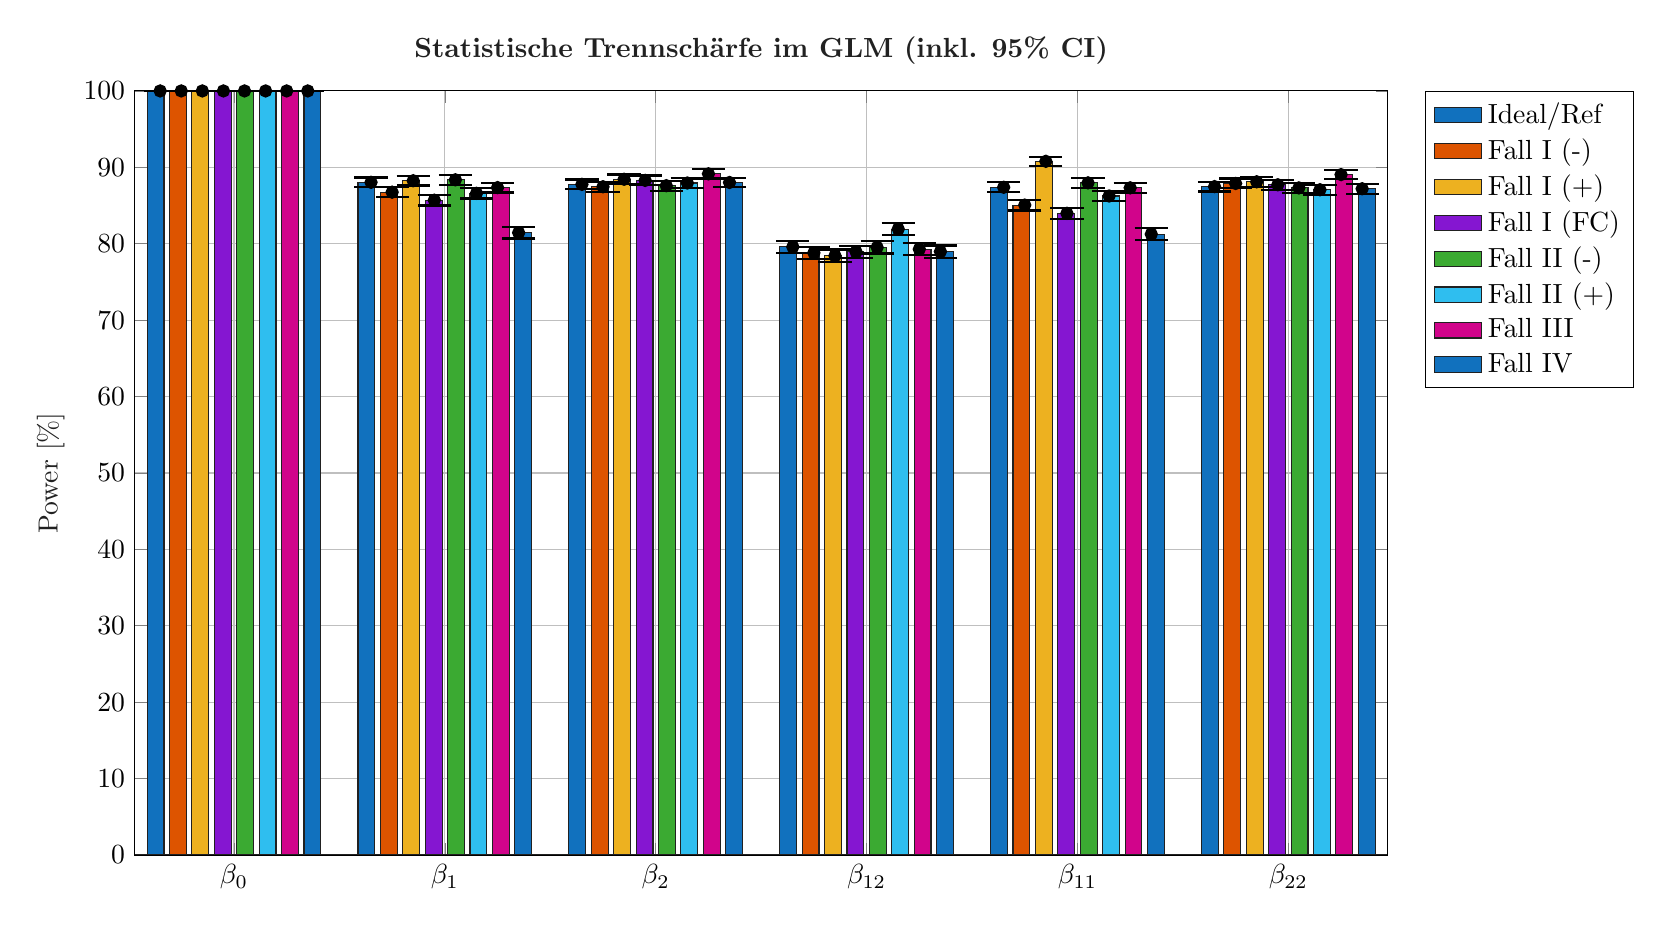
\begin{tikzpicture}

\begin{axis}[%
width=6.263in,
height=3.82in,
at={(1.051in,0.516in)},
scale only axis,
bar shift auto,
xmin=0.53,
xmax=6.47,
xtick={1,2,3,4,5,6},
xticklabels={{$\beta_0$},{$\beta_1$},{$\beta_2$},{$\beta_{12}$},{$\beta_{11}$},{$\beta_{22}$}},
ymin=0,
ymax=100,
ylabel style={font=\color{mycolor2}},
ylabel={Power [\%]},
axis background/.style={fill=white},
title style={font=\bfseries\color{mycolor2}},
title={\textbf{Statistische Trennschärfe im \ac{GLM} (inkl. 95\% CI)}},
xmajorgrids,
ymajorgrids,
legend style={at={(1.03,1)}, anchor=north west, legend cell align=left, align=left}
]
\addplot[ybar, bar width=0.08, fill=mycolor1, draw=mycolor2, area legend] table[row sep=crcr] {%
1	100\\
2	88.04\\
3	87.77\\
4	79.59\\
5	87.39\\
6	87.48\\
};
\addplot[forget plot, color=mycolor2] table[row sep=crcr] {%
0.53	0\\
6.47	0\\
};
\addlegendentry{Ideal/Ref}

\addplot[ybar, bar width=0.08, fill=mycolor3, draw=mycolor2, area legend] table[row sep=crcr] {%
1	100\\
2	86.75\\
3	87.46\\
4	78.81\\
5	85.06\\
6	87.89\\
};
\addplot[forget plot, color=mycolor2] table[row sep=crcr] {%
0.53	0\\
6.47	0\\
};
\addlegendentry{Fall I (-)}

\addplot[ybar, bar width=0.08, fill=mycolor4, draw=mycolor2, area legend] table[row sep=crcr] {%
1	100\\
2	88.25\\
3	88.44\\
4	78.43\\
5	90.79\\
6	88.11\\
};
\addplot[forget plot, color=mycolor2] table[row sep=crcr] {%
0.53	0\\
6.47	0\\
};
\addlegendentry{Fall I (+)}

\addplot[ybar, bar width=0.08, fill=mycolor5, draw=mycolor2, area legend] table[row sep=crcr] {%
1	100\\
2	85.7\\
3	88.29\\
4	78.93\\
5	83.98\\
6	87.72\\
};
\addplot[forget plot, color=mycolor2] table[row sep=crcr] {%
0.53	0\\
6.47	0\\
};
\addlegendentry{Fall I (FC)}

\addplot[ybar, bar width=0.08, fill=mycolor6, draw=mycolor2, area legend] table[row sep=crcr] {%
1	100\\
2	88.37\\
3	87.6\\
4	79.52\\
5	87.97\\
6	87.31\\
};
\addplot[forget plot, color=mycolor2] table[row sep=crcr] {%
0.53	0\\
6.47	0\\
};
\addlegendentry{Fall II (-)}

\addplot[ybar, bar width=0.08, fill=mycolor7, draw=mycolor2, area legend] table[row sep=crcr] {%
1	100\\
2	86.6\\
3	87.95\\
4	81.92\\
5	86.25\\
6	87.07\\
};
\addplot[forget plot, color=mycolor2] table[row sep=crcr] {%
0.53	0\\
6.47	0\\
};
\addlegendentry{Fall II (+)}

\addplot[ybar, bar width=0.08, fill=mycolor8, draw=mycolor2, area legend] table[row sep=crcr] {%
1	100\\
2	87.35\\
3	89.15\\
4	79.29\\
5	87.32\\
6	89.05\\
};
\addplot[forget plot, color=mycolor2] table[row sep=crcr] {%
0.53	0\\
6.47	0\\
};
\addlegendentry{Fall III}

\addplot[ybar, bar width=0.08, fill=mycolor1, draw=mycolor2, area legend] table[row sep=crcr] {%
1	100\\
2	81.44\\
3	88.02\\
4	78.97\\
5	81.25\\
6	87.2\\
};
\addplot[forget plot, color=mycolor2] table[row sep=crcr] {%
0.53	0\\
6.47	0\\
};
\addlegendentry{Fall IV}

\addplot [color=black, line width=0.8pt, only marks, forget plot]
 plot [error bars/.cd, y dir=both, y explicit, error bar style={line width=0.8pt}, error mark options={line width=0.8pt, mark size=6.0pt, rotate=90}]
 table[row sep=crcr, y error plus index=2, y error minus index=3]{%
0.65	100	0	0\\
1.65	88.04	0.636006681524652	0.636006681524652\\
2.65	87.77	0.642158667882012	0.642158667882012\\
3.65	79.59	0.789963137560228	0.789963137560228\\
4.65	87.39	0.650645580684292	0.650645580684292\\
5.65	87.48	0.648653286691743	0.648653286691743\\
};
\addplot [color=black, line width=0.8pt, only marks, forget plot]
 plot [error bars/.cd, y dir=both, y explicit, error bar style={line width=0.8pt}, error mark options={line width=0.8pt, mark size=6.0pt, rotate=90}]
 table[row sep=crcr, y error plus index=2, y error minus index=3]{%
0.75	100	0	0\\
1.75	86.75	0.664505763707133	0.664505763707133\\
2.75	87.46	0.649096961434884	0.649096961434884\\
3.75	78.81	0.800962555319536	0.800962555319536\\
4.75	85.06	0.698705334904493	0.698705334904493\\
5.75	87.89	0.639437166001477	0.639437166001477\\
};
\addplot [color=black, line width=0.8pt, only marks, forget plot]
 plot [error bars/.cd, y dir=both, y explicit, error bar style={line width=0.8pt}, error mark options={line width=0.8pt, mark size=6.0pt, rotate=90}]
 table[row sep=crcr, y error plus index=2, y error minus index=3]{%
0.85	100	0	0\\
1.85	88.25	0.631149673215474	0.631149673215474\\
2.85	88.44	0.626699510310962	0.626699510310962\\
3.85	78.43	0.806161867130913	0.806161867130913\\
4.85	90.79	0.566767442381794	0.566767442381794\\
5.85	88.11	0.634394777771696	0.634394777771696\\
};
\addplot [color=black, line width=0.8pt, only marks, forget plot]
 plot [error bars/.cd, y dir=both, y explicit, error bar style={line width=0.8pt}, error mark options={line width=0.8pt, mark size=6.0pt, rotate=90}]
 table[row sep=crcr, y error plus index=2, y error minus index=3]{%
0.95	100	0	0\\
1.95	85.7	0.686142785140236	0.686142785140236\\
2.95	88.29	0.630217236946118	0.630217236946118\\
3.95	78.93	0.799299222579379	0.799299222579379\\
4.95	83.98	0.718911221178248	0.718911221178248\\
5.95	87.72	0.643286690874294	0.643286690874294\\
};
\addplot [color=black, line width=0.8pt, only marks, forget plot]
 plot [error bars/.cd, y dir=both, y explicit, error bar style={line width=0.8pt}, error mark options={line width=0.8pt, mark size=6.0pt, rotate=90}]
 table[row sep=crcr, y error plus index=2, y error minus index=3]{%
1.05	100	0	0\\
2.05	88.37	0.628345278725002	0.628345278725002\\
3.05	87.6	0.645979843648391	0.645979843648391\\
4.05	79.52	0.790968581889319	0.790968581889319\\
5.05	87.97	0.637611558126105	0.637611558126105\\
6.05	87.31	0.652407397125446	0.652407397125446\\
};
\addplot [color=black, line width=0.8pt, only marks, forget plot]
 plot [error bars/.cd, y dir=both, y explicit, error bar style={line width=0.8pt}, error mark options={line width=0.8pt, mark size=6.0pt, rotate=90}]
 table[row sep=crcr, y error plus index=2, y error minus index=3]{%
1.15	100	0	0\\
2.15	86.6	0.667678538220303	0.667678538220303\\
3.15	87.95	0.638068811022761	0.638068811022761\\
4.15	81.92	0.754310679081239	0.754310679081239\\
5.15	86.25	0.67497388838384	0.67497388838384\\
6.15	87.07	0.657642097813089	0.657642097813089\\
};
\addplot [color=black, line width=0.8pt, only marks, forget plot]
 plot [error bars/.cd, y dir=both, y explicit, error bar style={line width=0.8pt}, error mark options={line width=0.8pt, mark size=6.0pt, rotate=90}]
 table[row sep=crcr, y error plus index=2, y error minus index=3]{%
1.25	100	0	0\\
2.25	87.35	0.651527556132509	0.651527556132509\\
3.25	89.15	0.609581269725375	0.609581269725375\\
4.25	79.29	0.79424653662701	0.79424653662701\\
5.25	87.32	0.652187636509617	0.652187636509617\\
6.25	89.05	0.612040403568261	0.612040403568261\\
};
\addplot [color=black, line width=0.8pt, only marks, forget plot]
 plot [error bars/.cd, y dir=both, y explicit, error bar style={line width=0.8pt}, error mark options={line width=0.8pt, mark size=6.0pt, rotate=90}]
 table[row sep=crcr, y error plus index=2, y error minus index=3]{%
1.35	100	0	0\\
2.35	81.44	0.762015735942507	0.762015735942507\\
3.35	88.02	0.636465932423724	0.636465932423724\\
4.35	78.97	0.798742469545723	0.798742469545723\\
5.35	81.25	0.765012254803804	0.765012254803804\\
6.35	87.2	0.65481602423887	0.65481602423887\\
};
\end{axis}
\end{tikzpicture}%